\section{Annex}
\begin{figure}[h!tpb]
    \centering
    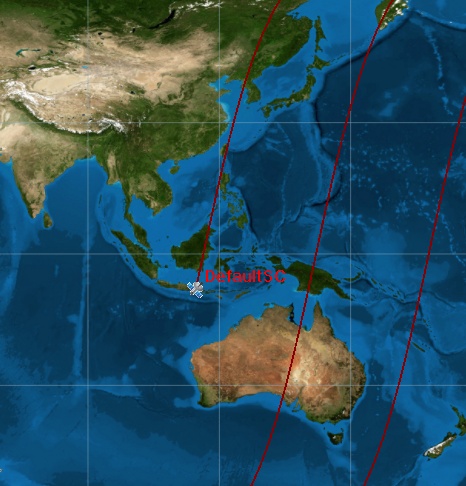
\includegraphics[width=\linewidth]{Figures/SatelliteGMAT.png}
    \caption{Satellite Mission Path}
    \label{fig:tcanther}
\end{figure}


\section{Annex}
\begin{figure}[h!tpb]
    \centering
    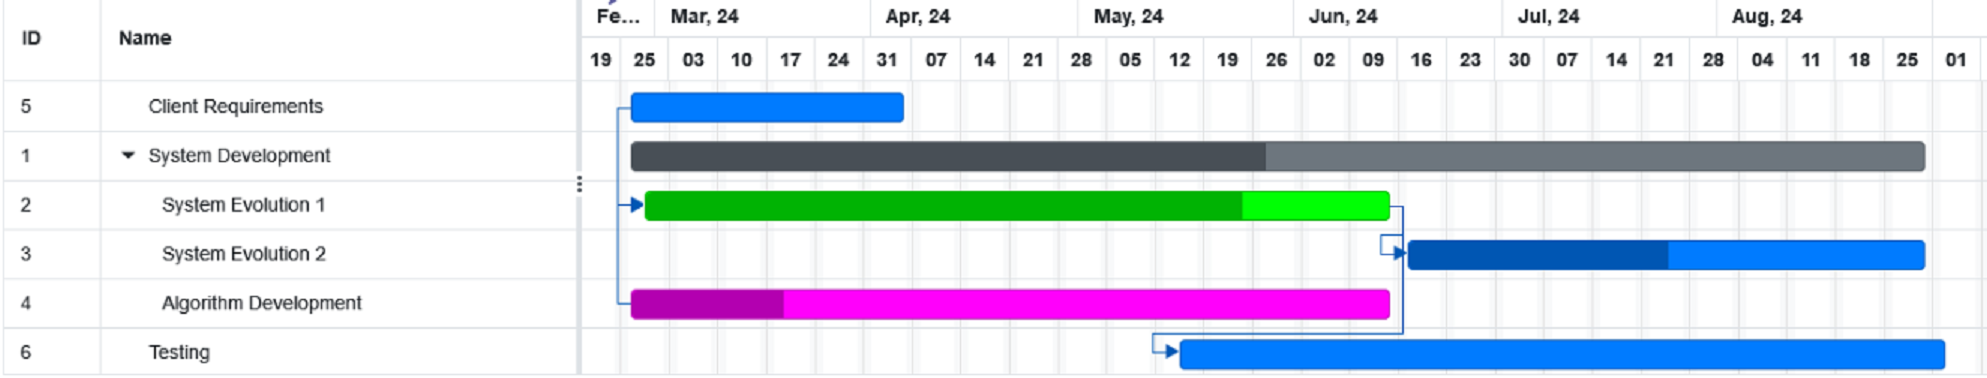
\includegraphics[width=\linewidth]{Figures/SatelliteSchedule.png}
    \caption{Project Schedule and Deliverables}
    \label{fig:tcanther}
\end{figure}


\begin{table}[h!]
    \centering
    \begin{tabular}{ccccll}
         Item&  Data Rate/Mbps&  Size/cm3& Mass/kg & Power/W&TLR\\
         Optical Camera&  60&  200& 0.3 & 10&9\\
         LiDAR&  10-20&  200& 0.3 & 15&9\\
         SAR&  50&  200& 0.3 & 20&9\\
         UV-IR&  20-40&  200& 0.3 & 5&7\\
 Total& 150-200& 800&1.2 & 50&8.5\\
    \end{tabular}
    \caption{Performance Budget}
    \label{tab:my_label}
\end{table}


\begin{table}
    \centering
    \begin{tabular}{p{0.25\linewidth} | p{0.75\linewidth}}
         Launch Phase& Coordinate with Launch provider and undergo initital depolyment and system checks\\
         Commissioning Phase& Detailed calibration of all instruments will be conducted to ensure they operate correctly. Baseline measurements taken.\\
         Operational Phase& Daily Routine Data collection with Periodic calibration and cross-validation with historical records\\
         Science Phase& Analysis and Distribution of Data to the Scientific Community.\\
         Decommissioning& Controlled Deorbiting\\
    \end{tabular}
    \caption{Mission Life Cycle}
    \label{tab:my_label}
\end{table}